\documentclass[11pt,psfig,times]{article}
\voffset=-2.2cm
\hoffset=-2.1cm

\setlength{\textwidth}{16.8cm}
\setlength{\textheight}{22.8cm}

\usepackage{latexsym}
\usepackage{epsfig}
\usepackage{times}
\usepackage{enumerate}
\usepackage{bm}
\usepackage{enumitem}
\usepackage{tikz}
\usepackage{amsthm, amsmath,amsfonts, amssymb}
\usepackage{algorithm,algorithmic}
\usepackage{tikz-network}
\usepackage{color}
\usepackage{tabularx}
\usepackage{float}
\usepackage{graphicx}
\usepackage{subcaption}

\usetikzlibrary{hobby}
\definecolor{lightblue}{RGB}{158,202,225}

\renewcommand{\thefootnote}{\fnsymbol{footnote}}
\renewcommand{\baselinestretch}{1.1}

\newcommand{\ignore}[1]{{}}
\newtheorem{theorem}{Theorem}[section]
\newtheorem{corollary}{Corollary}[section]
\newtheorem{lemma}{Lemma}[section]
\newtheorem{observation}{Observation}
\newtheorem{claim}{Claim}
\newtheorem{proposition}{Proposition}
\newtheorem{definition}{Definition}[section]
\newtheorem{fact}{Fact}


\begin{document}
\title{Near-Optimal Network Design with Selfish Agents}
\author{Nuo Xu\thanks {Department of Computer Science, Technical University of Munich. {\tt ge74mis@tum.de}}}
\date{25.11.2024}
\maketitle

\section{Introduction}

\subsection{Classic Generalized Steiner Tree and Steiner Forest problem}
In the classic generalized Steiner tree, we are given an undirected graph \(G = (V,E)\) with non-negative edge cost \(c_e \geq 0\) for every edge $c_e \in E$ and a set of terminals $R \subseteq V $. The goal is to compute the minimum-cost subgraph that spans all terminals. When the number of terminals is 2, it is the shortest path problem which can be solved in polynomial time using Dijkstra's problem. When the number of terminals equal to the number of vertices in the graph, it is the minimum spanning tree problem that can also be solved in polynomial time using Prim's algorithm. When $ 2 < |R| < |V|$, unless $P$ is equal to $NP$ there is no known polynomial algorithm to find the optimal solution for the Steiner tree problem.
\begin{figure}[H]
	\begin{center}
		\begin{subfigure}[b]{0.3\textwidth}
			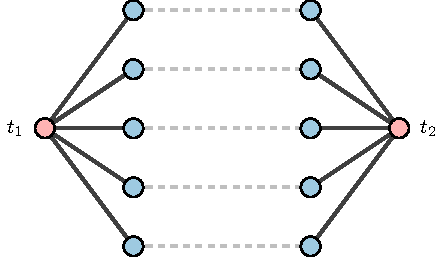
\includegraphics[width=\textwidth]{pictures/shortestpath.pdf}
			\caption{Shortest Path}
		\end{subfigure}
		\hspace{10pt}
		\begin{subfigure}[b]{0.25\textwidth}
			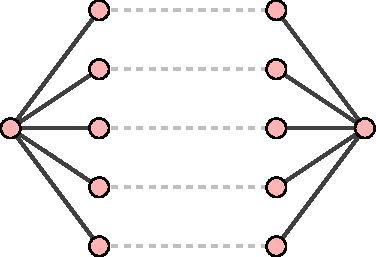
\includegraphics[width=\textwidth]{pictures/mst.pdf}
			\caption{Minimum Spanning Tree}
		\end{subfigure}
		\hspace{10pt}
		\begin{subfigure}[b]{0.25\textwidth}
			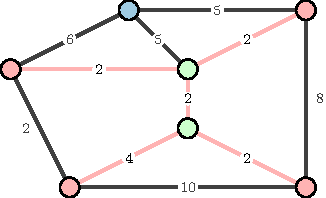
\includegraphics[width=\textwidth]{pictures/steinertree.pdf}
			\caption{Steiner Tree}
		\end{subfigure}
		\caption{Steiner tree problem with different number of terminals}
	\end{center}
\end{figure}
Similar as the Steiner tree problem, in the Steiner forest problem, we are given a collection of disjoint subsets of \(V: V_1,V_2,V_3,...V_n\). The goal is to compute a subgraph that any two vertices that belong to the same subset \(V_i\) are connected. The Steiner Tree problem is a Steiner Forest problem with a single subset of \(V\).  

\subsection{Introduction of Selfish Agents}
In real life, many networks are often developed and maintained by many selfish agents, for example, the Internet and traffic networks cross multiple countries. In such networks, agents tend to orient their behaviors to their own interests rather than the central optimal. Such selfish behaviors will potentially lead to a deviation from the central optimal. More specifically, given an undirected graph \(G\) with non-negative edge costs and \(N\) players, each player is interested in connecting a set of terminals (nodes in \(G\)) via buying a subgraph of \(G\). Players offer each edge in \(G\) certain amount of money, and they would like to pay a little as possible. For example, as shown in Fig \ref{fig:deviation}, both agents $t_1$ and $t_2$ would like to connect to the source $s$. The optimal solution clearly involves buying all edges except $t_1s$. However, if agents $t_1$ needs to pay more than $1+\epsilon$ for the optimal solution, they will just choose to pay for $t_1s$ and the total cost of the whole network will therefore be increased.

\begin{figure}[H]
	\begin{center}
	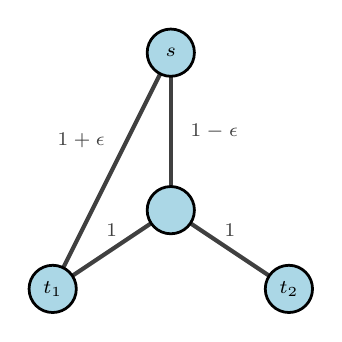
\begin{tikzpicture}
	\Vertex[label=$t_1$]{t1}
	\Vertex[label=$t_2$,x=3]{t2}
	\Vertex[x=1.5,y=1]{middle}
	\Vertex[x=1.5,y=3,label=$s$]{s}
	\Edge[label=$1$,position={above=1mm}](t1)(middle)
	\Edge[label=$1$,position={above=1mm}](t2)(middle)
	\Edge[label=$1-\epsilon$,position={right = 2mm}](s)(middle)
	\Edge[label=$1+\epsilon$,position={above left=2mm}](t1)(s)
	\end{tikzpicture}
	\end{center}
	\caption{An example of possible deviation from $OPT$.}
	\label{fig:deviation}
\end{figure}

\subsection{Formal Definition of Connection Game}
Here we formally define the connection game for \(N\) players as following:
\begin{itemize}
	\item An undirected graph \(G = (V,E)\).
	\item Non-negative edge cost \(c_e \geq 0\) for every edge $c_e \in E$.
	\item A subset of \(V\) for each player that they must connect to. 
	\item A payment function \(p_i\) indicates that player's payment strategy. \(p_i(e)\) is the contribution that player \(i\) would like to offer for edge \(e\).
\end{itemize}

If the sum of payment on certain edge \(e\) is larger than the cost on that edge \(c_e\), this edge is considered as bought and can be used by all players no matter they contribute to it or not. The goal of all players is to connect all of their terminals. If in the end, a player's terminates are not fully connected, they will face an infinite penalty.  

\section{Nash Equilibrium in Connection Game}
\subsection{Definition of Nash Equilibrium}
A crucial idea of modern game theory introduced by John von Neumann is the concept of \textit{mixed strategies}, which involves randomizing over pure strategies to optimize decision-making in competitive situations. This approach works particularly in \textit{zero-sum games}, where one player's gain is exactly balanced by the losses of other players. John Nash later expanded the scope of game theory significantly by introducing the concept of equilibrium in \textit{general \(N\)-player games}, demonstrating that every game with a finite number of players and strategies possesses at least one equilibrium point where no player can improve their payoff. 
\begin{theorem}[Nash's theorem]
	With randomization, any game with finite number of players and actions has a mixed-strategy of Nash equilibrium.
\end{theorem}
More specifically, the definition of Nash Equilibrium in Connection Game is defined as following:
\begin{definition}[Nash Equilibrium in Connection Game]
	A Nash equilibrium of the connection game is a payment function $p$ such that, if players offer payments \(p\), no payer has an incentive to deviate from their payment. 
\end{definition}
At first glance, if we allow players to pay fractional number, there will exist infinite number of strategies. Since we only have a finite number of players, we could say our game is a finite game without losing generality as long as we only allow payment function of each player to be rational number by scaling the cost of each edge from fractional to integer. Therefore, w.o.l.g connection game is indeed a finite game. According to Nash's theorem, any finite game has at least one mixed strategies Nash equilibrium but no grantee on pure strategy equilibrium. However, in the context of large-scale network creation, allowing players choosing their strategies randomly does not make much sense. We are also not interested in the expected payoff but a certain result.\textbf{ We are only interested in the pure Nash equilibrium in connection game.}

\subsection{Some Properties of Nash Equilibrium in Connection Game}
Here are some useful properties of the Nash equilibrium in connection game that can also be easily proved. 
\begin{itemize}
	\item \(G_p\) is a forest.
	\item Let \(T^i\) be the smallest tree in \(G_p\) connecting all terminals of player \(i\), then player \(i\) only contributes to edges in \(T^i\).
	\item Each edge is either bought or not at all. 
\end{itemize}
The first property holds as if there is a cycle in $G_p$, we could remove any edge without influencing any players' connectivity. Property 2 holds for similar reasons. If player $i$ is paying for any edges that are not in $T_i$, they are able to choose to not pay for those edges without influencing their connectivity. The last property is also easy to see as for any edge that is not fully paid, players that are paying for those edges can just choose to not pay at all without changing the final graph. 

According to these properties, we give the following game where pure equilibrium does not exist at all. As in shown in Fig \ref{fig:noequi}, there are two players. Player 1 wishes to connect node $s_1$ to node $t_1$ and similar for player 2. Suppose there exists a Nash equilibrium $p$. Then according to the first property $G_p$ must be a tree. Assume without losing generality, $G_p$ consists edge $s_1s_2$, $s_2t_1$, and $t_2t_1$. By the second property, player 1 and player 2 will only contribute to $s_1s_2$ and $t_2t_1$ respectively. This leaves the payment function of $s_2t_1$ to be decided. Clearly, player 2 already has their terminal and source connected and thus will not be willing to pay for anything else. At the same time, player 1 would have the incentive to not pay for $s_1s_2$ and only pay for $t_2t_1$. This situation will never end, and therefore no pure equilibrium will exist.

\begin{figure}
	\begin{center}
	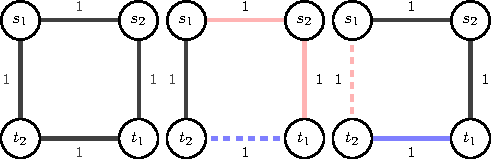
\includegraphics{pictures/noequi.pdf}
	\end{center}
	\caption{A game with no equilibrium at all}
	\label{fig:noequi}
\end{figure}

\begin{corollary}
Pure Nash equilibrium may not exist in the connection game.
\end{corollary}

    
\subsection{Fractional Nash Equilibrium}
Our life would be much simpler if we only let players choose to pay for an edge or not at all. However, some games require players to share costs on some edges for the existence of Nash equilibrium. We define such equilibrium as fractional Nash equilibrium.

\begin{definition}[Fractional Nash Equilibrium]If Nash equilibrium requires players to split cost of some edge, such Nash Equilibrium is fractional.	
\end{definition}

As shown in Fig \ref{fig:fracquil}, player 1 would like to connect $s_1$ to $t_2$ and similarly for player 2. Suppose edge $t_2t_1$ is not bought, then this leads to the case of no existence of equilibrium at all as shown in Fig \ref{fig:noequi}. Therefore, any equilibrium must involve buying edge $s_2t_2$. Suppose player 2 buys $s_2t_2$, player 1 would choose to buy $s_1t_2$ and edge $s_2t_1$ with total cost of 6. Then player 1 would have the incentive to pay 5 instead of 6 by either buying edge $s_1s_2$ or $t_2t_1$ instead of $s_2t_2$. This leads to a similar case to Fig \ref{fig:noequi}. Suppose player 2 does not choose to buy $s_2t_2$, the only response for which player 1 would not deviate would be either buying edge $s_1t_2$ and $t_2t_1$ or $s_1s_2$ and $s_2t_1$. Either way player 2 is still not connected. They would like to buy the corresponding edge that costs 3. This again leads to the same case with no equilibrium at all. To archive an equilibrium in such game, the cost of edge $s_2t_2$ must be shared. It can be easily verified that the strategy where player 1 paying fully for edges $s_1t_2$ and $s_2t_1$ and paying 1 for $s_2t_2$ while player 2 paying 5 for $s_2t_2$ is indeed an equilibrium.
\begin{figure}[H]
\begin{center}
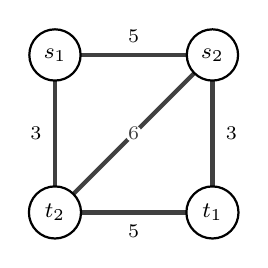
\begin{tikzpicture}
	\coordinate (s1) at (0,0);
	\coordinate (s2) at (2,0);
	\coordinate (t2) at (0,-2);
	\coordinate (t1) at (2,-2);

	\node[draw,circle,fill=white,thick,minimum size=2pt] (CircleNode) at (s1){\footnotesize $s_1$};
	\node[draw,circle,fill=white,thick,minimum size=2pt] (CircleNode) at (s2){\footnotesize $s_2$};
	\node[draw,circle,fill=white,thick,minimum size=2pt] (CircleNode) at (t1){\footnotesize $t_1$};
	\node[draw,circle,fill=white,thick,minimum size=2pt] (CircleNode) at (t2){\footnotesize $t_2$};

	\Edge[label=$5$,fontcolor=black,position={above=1mm}](s1)(s2)
	\Edge[label=$3$,fontcolor=black,position={right=1mm}](s2)(t1)
	\Edge[label=$5$,fontcolor=black,position={below=1mm}](t1)(t2)
	\Edge[label=$3$,fontcolor=black,position={left=1mm}](t2)(s1)
	\Edge[label=$6$](t2)(s2)
\end{tikzpicture} 
\end{center}
\caption{Fractional Nash Equilibrium}
\label{fig:fracquil}
\end{figure}


\subsection{Price of Anarchy and Stability}
As mentioned in Section 1, the introduction of selfish agents can lead to worse equilibrium than the best centralized optimum. The question is how bad an equilibrium can be. Here we introduce the concept of \textit{price of anarchy} to measure the badness of an equilibrium.
\begin{definition}[Price of Anarchy] The price of anarchy of connection game is defined as the ratio of the cost of worst Nash equilibrium over the optimal centralized design.
	\[P_A = \dfrac{\text{cost of the worst equilibrium} }{\text{cost of OPT}}\]
\end{definition}

It turns out the price of anarchy can easily be as bad as $N$ in a simple network as in Fig \ref{fig:anarchyN}. In such network, every player has the same source $s$ and terminal $t$. In between of $s$ and $t$, there exist two route both directly connect $s$ to $t$ with one only cost 1 and the other costs $N$. The worst equilibrium is that every player pays 1 for the route with cost of $N$. And none of them will have the incentive to switch to the route with cost of 1 as that will not reduce their final payment. Such payment function is indeed an equilibrium the corresponding price of anarchy is $N$.
\begin{corollary}
The price of anarchy can be as bad as \(N\).
\end{corollary}

\begin{figure}[H]
	\begin{center}
	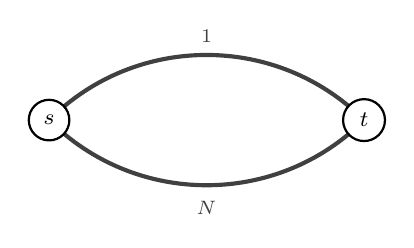
\begin{tikzpicture}
	\coordinate (s1) at (0,0);
	\coordinate (s2) at (4,0);
	\node[draw,circle,fill=white,thick,minimum size=2pt] (CircleNode) at (s1){\footnotesize $s$};
	\node[draw,circle,fill=white,thick,minimum size=2pt] (CircleNode) at (s2){\footnotesize $t$};
	\Edge[label=$1$,position={above=1mm},bend=45](s1)(s2)
	\Edge[label=$N$,position={below=1mm},bend=-45](s1)(s2)
	\end{tikzpicture}
	\end{center}
	\caption{A game with price of anarchy of $N$.}
	\label{fig:anarchyN}
\end{figure}

Although the price of anarchy in such game can be pretty high, it is also easy to see that the best equilibrium can be as good as the $OPT$ where each player pays $1/N$ to the route with cost of 1. Therefore, the complementary concept of price of stability becomes more of our interests, which evaluate how good the best equilibrium can be.
\begin{definition}[Price of Stability] The price of stability of connection game is defined as the ratio of the cost of best Nash equilibrium over the optimal centralized design.
	\[P_S = \dfrac{\text{cost of the best equilibrium} }{\text{cost of OPT}}\]
\end{definition}

\section{Single Source Games}
\subsection{Definition of Single Source Games}
We have already known that pure Nash Equilibrium might not exist in the general version of connection game as shown in Fig \ref{fig:noequi}. However, in the single source connection game, Nash equilibrium is determined to exist. In the single source game, we only allow every player \(i\) has one unique terminal \(t_i\)that they all would like to connect a common terminal \(s\). This can be considered as a special version of Steiner tree problem where \(R = \{s,t_0,t_1,...t_N\}\). 

\begin{definition}[Single source Game]
	A single source game is a game in which all players share a common terminal \(s\) and in addition, each player \(i\) has exactly one other terminal \(t_i\).
\end{definition}

As we have talked before, it is not much of our interests to study the worst equilibrium as it can be as bad as $N$. Therefore, we would like to instead see how good the best equilibrium can be. One natural question to ask is that can we achieve an equilibrium that equals to the \(OPT\)? The answer is yes. Suppose the minimum cost Steiner tree \(T^*\) that spans over all players' terminals and $s$ is given on a sliver plate, we are going to derive an algorithm that gradually assigns each player \(i\) a payment strategy on edge \(e\). Then we are going to prove that the final payment function \(p\) will fully pay for $T^*$ and end up as an equilibrium, thus yield price of stability as 1.  

\subsection{Payment Strategy Design}
Possible common strategies like \textit{Sharply Value} and \textit{Marginal Cost} both fail at archiving equilibrium in the connection game. Take Fig \ref{fig:deviation} as an example, if we use Sharply Value to decide $p_i(e)$, player 1 and 2 will need to share the cost of edge $1-\epsilon$ evenly, which will lead player 1 to deviate. 

The intuition behind algorithm \ref{alg:1} is to assign payment function on edges that we know for sure which players are interested in. Let \(T^*\) be rooted from \(s\). We will visit \(T^*\) in reverse breadth-first-search order. For every edge \(e\), suppose \(e\) is removed from \(T^*\), \(T^*\) will be divided into two subtrees. As shown in Fig \ref{fig:tets}, let the subtree that does not contain \(s\) be \(T_e\) and the one contains \(s\) be \(T_s\). It is clear that players in \(T_s\) would not be interested in paying anything for \(e\) as not including \(e\) in the final graph will not affect their connection to \(s\) at all. Therefore, when traversing \(T^*\) in reserve BFS order, for every player \(i \in T_e\) we determine \(p_i(e)\).

\begin{figure}[H]
	\begin{center}
		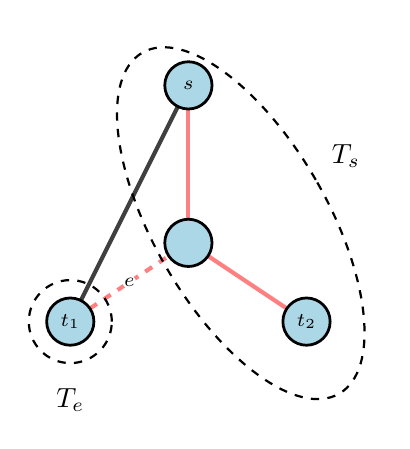
\begin{tikzpicture}
			\Vertex[label=$t_1$]{t1}
			\Vertex[label=$t_2$,x=3]{t2}
			\Vertex[x=1.5,y=1]{middle}
			\Vertex[x=1.5,y=3,label=$s$]{s}
			\Edge[style={dashed},label=$e$,color=red!50,fontcolor=black](t1)(middle)
			\Edge[color=red!50](t2)(middle)
			\Edge[color=red!50](s)(middle)
			\Edge(t1)(s)
			\draw[dashed,thick](0,0) circle (15pt);
			\node at (0, -1) {$T_e$};
			\draw[dashed,thick,rotate=30,label=$T_s$](2.5,0) ellipse(1.1cm and 2.5cm);
 			\node at (3.5, 2.1) {$T_s$};
		\end{tikzpicture}
	\end{center}
	\caption{$T_e$ and $T_s$}
	\label{fig:tets}
\end{figure}

In every iteration, we modify the cost of every edge according to the following rules: edges \(e \in T_e\) cost \(p_i(e)\); edges \(e \in T_s\) costs 0;edges \(e\notin T^*\) stay the same. Then we find the cheapest alternative path \(A_i\) from \(t_i\) to \(s\) from \(G \setminus \{e\}\) under modified cost which can be done in polynomial time. Compare the following two values, and we just assign $p_i(e)$ as the minimum one. 
		\begin{itemize}
			\item $c(e) - $ contribution from other players to edge \(e\)
			\item cost of \(A_i-\) sum of all contribution of player \(i\) to \(T^*\) 
		\end{itemize}

When deciding player $i$'s payment function $p_i(e)$ for edge $e$, it must be the case that payment functions for all edges in $T_e$ have already been bought. So if player $i$ use any edges in $T_e$, we can just assume that the cost will stay the same as $p_i(e)$. By changing the cost of edges in $T_s$, we ensure that players in $T_e$ never pay for the future and leave the decision in later iteration. A detailed pseudocode is presented here:
\begin{algorithm}[H]
	\begin{algorithmic}[1]
		\STATE $p_i(e) \gets 0, \forall t_i \in R, \forall e \in E$ 
		\WHILE{$e \in ReverseBFS(T^*)$}
		\IF{$e$ is a cut} 
		\STATE $p_i(e) \gets c(e)$
		\ELSE
		\STATE \(c(e) \gets p_i(f)  \qquad \forall e \in T_e\) 
		\STATE \(c(e) \gets 0 \qquad \forall e \in T_S\) 
		\STATE $A_i \gets$ the cheapest alternative path from \(s\) to \(t_i\) in $G\setminus\{e\}$ 
		\STATE \(p_i(e) \gets min\{c(A_i) - \sum_{e\in T^*}p_i(e), c(e)-\sum_{j}p_j(e) \}\)
		\ENDIF
		\ENDWHILE
	\end{algorithmic}
	\caption{pseudocode for assigning $p_i(e)$ }
	\label{alg:1}
	\end{algorithm}
	
\begin{corollary}
	If in the end of the game $T^*$ is successfully fully paid, the final payment function is indeed a Nash equilibrium and the price of anarchy will be 1.
\end{corollary}
Consider the cost player \(i\) needs to pay if they choose to deviate, \(c(A_i) - \sum_{f\in T^*}p_i(T^*)\), and \(c(e) - \sum_{j\in T_i,j\neq i}p_j(e)\). By choosing the minimum between these two values, we ensure that player \(i\) will never contribute to \(e\) more than the cost of deviation. In another word, it is always cheaper for players to stay in \(T^*\). This holds true for every player in every edge in $T^*$. Therefore, \(p\) is indeed a Nash equilibrium. 

\subsection{Proof of $T^*$ Being Fully Paid}

To prove that every edge in \(T^*\) is fully paid in the end, first we are going to assume that the following lemma is true:

Suppose \(A_i\) is \(i\)'s alternative path at some stage of the algorithm. Then suppose there are two nodes \(v\) and \(w\) on \(A_i\) that divides this path into three parts. Let edges on \(A_i\) from \(t_i\) to \(v\) be \(f_1\), from \(v\) to \(w\) be \(f_2\), from \(w\) to \(s\) be \(f_3\). As shown in Fig \ref{fig:lemma3.1}, the blue part is $T_e$ and the red part is $T_s$. 
	\begin{lemma}
		There must exist a pair of \(\{v,w\}\) such that \(f_1 \in T_e\), \(f_2 \notin T^*\), \(f_3 \in T_s\).
	\end{lemma}

\begin{figure}[H]
\begin{center}
	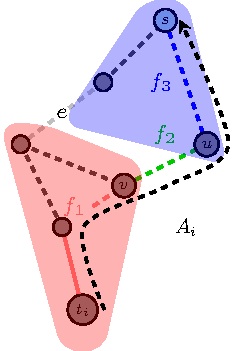
\includegraphics{pictures/lemma3.1.pdf}
	\end{center}
	\caption{Lemma 3.1}
	\label{fig:lemma3.1}
\end{figure}

Suppose there exists some edge \(e\) such that after all players in \(T_e\) have contributed to that edge, \(p_i(e) < c(e)\), we can prove $T^*$ is fully bought by showing that \(T_e\) costs more than \(\bigcup_{i\in T_e} A_i\) which is a contradiction to the fact that \(T^*\) is \(OPT\).

	\begin{lemma}
		All edges in \(T^*\) are bought, i.e. $\sum p_i(e) = c(e)$ for any $e \in T^*$.
	\end{lemma}
	
	\begin{figure}[H]
		\begin{center}
		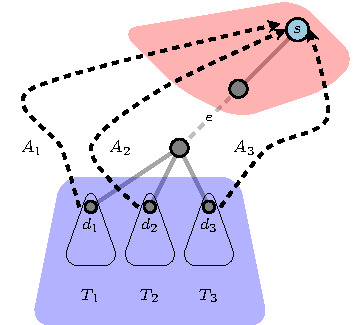
\includegraphics{pictures/lemma3.2.pdf}
		\end{center}
		\caption{Lemma 3.2}
		\label{fig:Lemma3.2}
	\end{figure}
			
 Suppose in the end of the game, edge $e$ is not fully paid. Since in each step when we decide a payment $p_i(e)$ for player $i$ on $e$, we choose \(p_i(e) \gets min\{c(A_i) - \sum_{e\in T^*}p_i(e), c(e)-\sum_{j}p_j(e) \}\), if we decide player $i$ needs to pay $c(e)-\sum_{j}p_j(e) $, then $e$ is bought. Therefore, we must set all players in $T_e$, their payment function on $e$ to be $c(A_i) - \sum_{e\in T^*}p_i(e)$. If we modify $T^*$ by replacing $T_e$ with \(\bigcup_{i\in T_e} A_i\), all other players leave their payments unchanged and all $A_i$ can be fully paid. By \textbf{Lemma 3.1}, we know that all players in $T_e$ can stay connect to $s$ after the modification without increasing their expenditures. \textbf{This is a contradiction to $T^*$ being unique.}

\subsection{Proof of Lemma 3.1}
Suppose once $A_i$ reaches a node in $T_s$, then all subsequent edges will be in $T_s$ as edges in $T_s$ cost 0 under modified cost. Since $s \in T_s$, $A_i$ will always reach a node in $T_s$. Therefore, to prove \textbf{Lemma 3.1} we only need to prove that if $A_i$ leaves $T_e$ it will only be in $G\setminus T_e$, i.e. \textbf{$A_i$ does not go back to $T_e$ anymore.} We show this by contradiction. 

As shown in Fig \ref{fig:alterpath}, suppose there are two nodes \(v\) and \(w\) on \(A_i\) that divides the part of $A_i$ before reaching to $T_s$ into three parts such that \(P_1 \in T_e\), \(P_2 \notin T^*\), \(P_4 \in T_e\). Let $y$ be the lowest common ancestor of $t_i \text{ and } w \text{ in } T_e$. Define $P_3$ to be the path from $t_i$ to $y$ in $T_e$. We will show that by replacing $P_1 \bigcup P_2$ with $P_3 \bigcup P_4$, player $i$ would obtain a better deviation than $A_i$.
		\begin{figure}		
		\begin{center}
		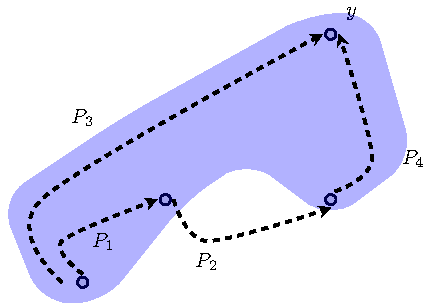
\includegraphics{pictures/alterpath.pdf}
		\end{center}
		\caption{Alternative path structure in the proof of Lemma 3.1}
		\label{fig:alterpath}
	\end{figure}

First, we claim that the modified costs for edges on $P_4$ are always 0 since none of them are on player $i$'s path from $t_i$ to $s$ in $T^*$.
		\begin{claim}
			$ c^{'}(P_4) = p_i(P_4) = 0$ for $i$.
		\end{claim}
Secondly, we can observe that $P_1$ is always restrictly below $y$. If this is not the case, $P_3$ is just a subpath of $P_1$. Since $c^{'}(P_3) \leq c^{'}(P_1) \text{ and } c^{'}(P_4) = 0$, we get $ c^{'}(P_3\bigcup P_4) \leq c^{'}(P_1\bigcup P_2)$ as desired.  	
		\begin{claim}
		$P_1$ is restrictly below $y$,i.e. $P_1$ is a subpath of $P_3$. 
		\end{claim}

In the case that $P_1$ is restrictly below $y$,
when deciding the payment of each edge in $P_3$, $p_i(e) \leq c(A_i)$. At any time, player $i$'s payments are upper bounded by the modified cost of his alternate path, which is in turn upper bounded by the modified cost of any path from $t_i$ to $s$. 
			 \[ c^{'}(P_3\bigcup P_4) = c^{'}(P_3) \leq c^{'}(P_1\bigcup P_2)\]
	
We finished proving the following theorem:
		\begin{theorem}
			For every single source game, there always exists a Nash equilibrium with price of stability being 1.
		\end{theorem}
	
\section{Approximate Nash Equilibrium in Connection Game}
	Although we proved that the determined existence of Nash equilibrium in single source game, \textbf{the algorithm presented is not feasible} as the finding the minimum cost Steiner tree is NP-hard by itself.  Moreover, the Steiner tree problem is APX-hard, meaning that it is hard to approximate within any constant factor. In fact, it has been proven that it is NP-hard to approximate Steiner tree problem within ratio \(96/95\). 
		
		\begin{fact}
			Steiner Tree problem is APX-hard, i.e. there exists a constant $\alpha$ such that $c(T) = \alpha c(T^*)$.
		\end{fact}
		
	If we are given an approximated Steiner tree \(T\) and try to use the same algorithm to assign \(p_i(e)\) in \(T\), since \(T\) is not optimal, there will be some edge \(e\) that players are unwilling to pay for.Therefore, we can only hope to archive an $\epsilon$-equilibrium on the approximated Steiner Tree. In game theory, a Nash equilibrium is an equilibrium that every player's regret is equal to 0. An $epsilon$-equilibrium is an equilibrium where every player's regret is less or equal to $\epsilon$. A specific definition of approximate equilibrium of connection game is defined as following:
		\begin{definition}[Approximate Equilibrium]
			A \((1+\epsilon)\)-approximate Nash Equilibrium is a payment function \(p\) such that player \(i\) would not deviate their payment by a factor of \(1+\epsilon\), i.e. let $ p_i^{'}(T)$ be player's final payment,$ p_i^{'}(T) \leq (1+\epsilon)p_i(T)$.
		\end{definition}
		
	
		\begin{theorem}
			Given a single source game and \(\alpha\) approximation of minimum-cost Steiner tree \(T\), \(\forall \epsilon > 0\), there is a polynomial algorithm which return a \((1+\epsilon)\)-approximation \textit{Nash equilibrium} on Steiner Tree \(T^{'}\), where $c(T^{'}) \leq c(T)$.
		\end{theorem}
	
	Now suppose instead of trying to fully pay every edge on the approximated Steiner tree we reduce the cost of every edge by $\gamma$. If in the end of the game all players end of buying  $T$ with $\gamma$ reduction, we can increase their final payment $p_i^{'}(e)$ by $\gamma\frac{p_i(T)}{P(T)}$. $T$ will be full paid, and it is a $(1+\epsilon)$ Nash Equilibrium. We can derive the value $\gamma$ as following to ensure that this will be a $1+ \epsilon$ approximation. Suppose there are $m$ edges in $T$,
	\[p_i^{'}(T) - p_i(T) \leq \epsilon p_i(T)\]
	\[p_i^{'}(T) - p_i(T) =  \gamma\frac{p_i(T)}{P(T)}m =  \gamma\frac{p_i(T)}{c(T)-m\gamma}m \leq \epsilon p_i(T)\]
	\[ \frac{m\gamma}{c(T)-m\gamma} \leq \epsilon \Rightarrow \gamma \leq \frac{\epsilon c(T)}{(1+\epsilon)m}\]
	Since $T$ is not optimal, it is possible that agents will not be willing to pay for $T$ even we reduce the cost on every edge in $T$. What we do instead is to form a cheaper tree. Therefore, we need to define $\gamma$ in a way that even after reconstruction, the final payment will still be a $1+\epsilon$ approximation. 
	
	Suppose the reconstructed tree $T^{'}$ has $m^{'}$ edges, we want $\gamma$ is also less or equal to $\frac{\epsilon c(T^{'})}{(1+\epsilon)m^{'}}$. As $T \text{ and } T^{'}$ are both trees, $m \text{ and } m^{'}$ will both be smaller that the number of vertices in the original graph.  Because $c(T^{'}) \geq c(T^*) = \frac{c(T)}{\alpha}$, we can define $\gamma$ as:
	\[\gamma = \frac{\epsilon c(T)}{(1+\epsilon)n\alpha},\quad n = |V|\]
	
	
		\begin{algorithm}[H]
			\begin{algorithmic}[2]
				\STATE $c^{'}(e) \gets  c(e) -\gamma \quad \forall e \in T$
				\STATE Run Algorithm 1 to attempt to pay for on $T$ under modified cost
				\WHILE{\( e \in T \) }
				\IF{\(e\) is not fully paid}
				\STATE  Adjust \( T\) by replacing \(T_e\) with  \(\bigcup_{i\in T_e} A_i\) to get \(T^{'}\)
				\STATE BREAK
				% Run Algorithm 1 to pay for $T^{'}$ under modified cost
				\ENDIF
				\ENDWHILE
				\STATE Modify($T^{'}$)
			   
			\end{algorithmic}
			\caption{Modify $T$ }
			\end{algorithm}
		
		% 	$P(T^{'}) \gets \sum_i p_i(T^{'})$\\
		% 	$p_i^{'}(e) \gets p_i(e) + \gamma\frac{p_i(T^{'})}{P(T^{'})}\quad \text{ for all players and every } e \in T^{'}$
	
		% 
		At the end of the algorithm, we increase player $i$'s payment on edge $e$ proportionally to their contribution to $T^{'}$, \[p_i^{'}(e) = p_i(e) + \gamma\frac{p_i(T^{'})}{P(T^{'})}\]
	
		\begin{claim}
			This algorithm fully pays for $T^{'}$ and runs in polynomial time.
		\end{claim}
	
		Clearly $T^{'}$ is fully paid as $\sum_i p_i^{'}(e) = \sum_i p_i(e) + \gamma$. Whenever \( e \in T \) is not fully paid, we form a new tree $T^{'}$, and $c(T^{'}) \leq c(T) - \gamma $. Therefore, we need to reconstruct our Steiner tree most  $\frac{c(T)}{\gamma} = \frac{(1+\epsilon)n\alpha }{\epsilon}$ times.

		\begin{lemma}
			$P^{'}(T^{'})$ Is A $(1+\epsilon)$ Nash Equilibrium
		\end{lemma}
		To prove that the final payment is an equilibrium, suppose $T^{'}$ has $m^{'}$ edges:
		\[p_i^{'}(T^{'}) = p_i(T^{'}) + \gamma\frac{p_i(T^{'})}{P(T^{'})}m^{'} = p_i(T^{'}) + \gamma\frac{p_i(T^{'})}{c(T^{'}) - m^{'}\gamma}\]
		\begin{align*}
		p_i^{'}(T^{'}) - p_i(T^{'}) &=  \gamma\frac{p_i(T^{'})}{c(T^{'}) - m^{'}\gamma}m^{'} = \frac{\epsilon c(T) p_i(T^{'}) m^{'} }{(1+\epsilon)n\alpha(c(T^{'}) - m^{'}\gamma)}  \\ &=  \frac{\epsilon c(T) p_i(T^{'})}{(1+\epsilon)\alpha n(\frac{c(T^{'})}{m^{'}} - \gamma)} =  \frac{\epsilon c(T) p_i(T^{'})}{(1+\epsilon)\alpha (\frac{n}{m^{'}} - \frac{n\gamma}{c(T^{'})})c(T^{'})}   
		\end{align*}
		Substitute the definition of $\gamma$ into the equation again, we get
		\[\frac{n\gamma}{c(T^{'})} = \frac{\epsilon c(T) n}{(1+\epsilon)n\alpha c(T^{'})} = \frac{\epsilon c(T) }{(1+\epsilon)\alpha c(T^{'})}\]
		Since $c(T) = \alpha c(T^*)$, we get \[ \frac{n\gamma}{c(T^{'})} = \frac{\epsilon c(T^*)}{(1+\epsilon)c(T^{'})} < \epsilon\]
		As $\frac{n}{m^{'}} > 1$, we get
		\[p_i^{'}(T^{'}) - p_i(T^{'}) \leq \frac{\epsilon c(T) p_i(T^{'}) }{(1+\epsilon)\alpha (1-\epsilon) c(T^{'}) } = \frac{\epsilon  p_i(T^{'}) }{(1+\epsilon) (1-\epsilon) } \leq \epsilon p_i(T^{'})\]
	
		
\section{Lower Bound of Approximate Nash Equilibrium in General Case}
	
\subsection{General Game}
In the general case, players can have different numbers of terminals and do not necessarily share the same source.

\begin{lemma}
	The price of stability in general cases can be bad as $\Theta(N)$.
\end{lemma}

As shown in the figure, each player $i$ owns terminals $s_i$ and $t_i$. The optimal centralized solution has cost $1 + 3\epsilon$ involves edge from $s_3,....s_N$ to $t_3,....t_N$ and any three edges with cost of $\epsilon$. However, if the path of length 1 were bought, each player $3...N$ will not be willing	to pay for any edge that costs $\epsilon$. And the situation of players 1 and 2 reduces to the example in Section 2	of a game with no Nash equilibrium at all. Therefore, any possible equilibrium will end up paying $N-2$.

\begin{figure}[H]
\begin{center}	
	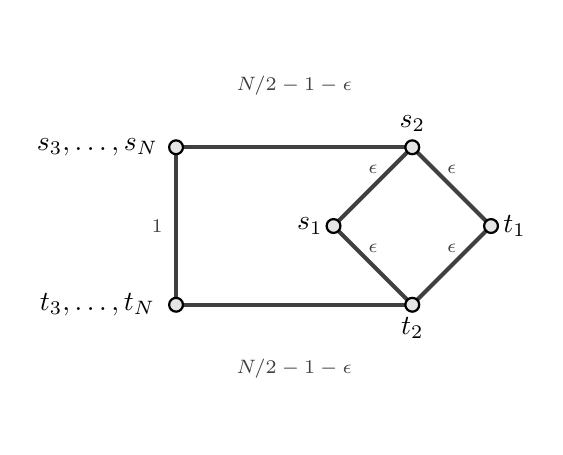
\begin{tikzpicture}
		\coordinate (s) at (0,0);
		\coordinate (t) at (0,-2);
		\coordinate (s1) at (2,-1);
		\coordinate (t1) at (4,-1);
		\coordinate (s2) at (3,0);
		\coordinate (t2) at (3,-2);
		\node[draw,circle,fill=gray!20,thick,inner sep=1pt,minimum size=5pt] (CircleNode) at (s)  {};
		\node[draw,circle,fill=gray!20,thick,inner sep=1pt,minimum size=5pt] (CircleNode) at (s1)  {};
		\node[draw,circle,fill=gray!20,thick,inner sep=1pt,minimum size=5pt] (CircleNode) at (s2)  {};
		\node[draw,circle,fill=gray!20,thick,inner sep=1pt,minimum size=5pt] (CircleNode) at (t)  {};
		\node[draw,circle,fill=gray!20,thick,inner sep=1pt,minimum size=5pt] (CircleNode) at (t1)  {};
		\node[draw,circle,fill=gray!20,thick,inner sep=1pt,minimum size=5pt] (CircleNode) at (t2)  {};
		\Edge[label=$1$,position={left=1mm}](s)(t)
		\Edge[label=$N/2-1-\epsilon$,position={above=0.1pt}](s)(s2)
		\Edge[label=$\epsilon$,position={above=1mm}](s1)(s2)
		\Edge[label=$\epsilon$,position={above=1mm}](s2)(t1)
		\Edge[label=$\epsilon$,position={above=1mm}](t1)(t2)
		\Edge[label=$\epsilon$,position={above=1mm}](t2)(s1)
		\Edge[label=$N/2-1-\epsilon$,position={below=1pt}](t)(t2)
		\node at  ([shift={(-1,0)}]s) {$s_3,\dots,s_N$};
		\node at  ([shift={(-1,0)}]t) {$t_3,\dots,t_N$};
		\node at ([shift={(-0.3,0)}]s1) {$s_1$};
		\node at ([shift={(0.3,0)}]t1) {$t_1$};
		\node at ([shift={(0,0.3)}]s2) {$s_2$};
		\node at ([shift={(0,-0.3)}]t2) {$t_2$};
	\end{tikzpicture}
	\end{center}
	\caption{A game with high price of stability}
\end{figure}
	
	\subsection{Lower Bounds on Nash Equilibrium in General Case}
	Since the price of stability can be as bad as $\Theta(N)$ and pure Nash equilibrium may not exist at all, we cannot hope to be able to provide cheap Nash equilibrium for multi-source games. Therefore, we instead hope that we can get a cheap $(1+\epsilon)$-approximate equilibrium. It turns out the best $epsilon$ we can hope for is no less than $\frac{1}{2}$.

	\begin{theorem}
		There exists such a graph that any equilibrium that purchases the optimal Steiner forest is at least a $(3/2-\epsilon)$ approximate equilibrium for any $\epsilon > 0$.
	\end{theorem}
	
	To prove \textbf{Theorem 5.1}, we construct a graph as following requirements. First we start with a cycle with $2N$ vertices from $v_1 \text{ to } v_{2N}$ clockwise. For $v_i$, add an edge from vertex $i$ to vertex $(i+N-1)mod (2N)$ and an edge with cost 1 from vertex $i$ to $(i+N+1)mod (2N)$. Then we add $N$ players and each of them have a source $s_i$ and a terminal $t_i$. Let vertices from $v_1$ to $v_N$ be the $s$ for each player and vertices $v_{N+1}$ to $v_{2N}$ be the terminals.	Fig \ref{fig:generalgame} is an example of such graph with 5 players.
			   
	\begin{figure}[H]
		\begin{center}
			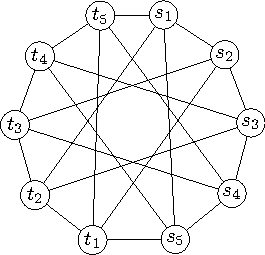
\includegraphics{pictures/generalcase.pdf}
		\end{center}
		\caption{ Example of the constructed graph with 5 players.}
		\label{fig:generalgame}
	\end{figure}

	It is clear that in such graph optimal central design costs $2N-1$ with all the edges in the outer cycle with edge from $s_1$ to $t_N$. Therefore, we need to prove that any equilibrium will cost at least $(3/2)*(2N-1)$.
	
	Suppose there is an equilibrium that is better than $3/2$, we can derive that player 1 and player $N$ will not be willing to pay for more 3 for this graph. 

	\begin{lemma}
		For any equilibrium that is better than $3/2$, player 1 and player $N$ will not be willing to pay for more 3 for this graph.
	\end{lemma}
	As shown in Fig \ref{fig:3/2equi}, suppose player 1 pays $x$ t the path from $s_1 \rightarrow t_1$ and $y$ to the path $t_1 \rightarrow t_N$. Two possible incentive choices for player 1 are either to pay for only the path from $s_1 \rightarrow t_1$ or the path from $s_1 \rightarrow t_1$ and an additional edge $t_Ns_1$. If the equilibrium is a $3/2$ equilibrium, then the following inequalities must hold true \[\frac{x+y}{x} \leq \frac{3}{2}\quad \text{ and }\quad\frac{x+y}{y+1} \leq \frac{3}{2}\]
	Therefore, we get $x+y\leq 3$.
	
	\begin{figure}
		\begin{center}
			\begin{subfigure}[b]{0.3\textwidth}
				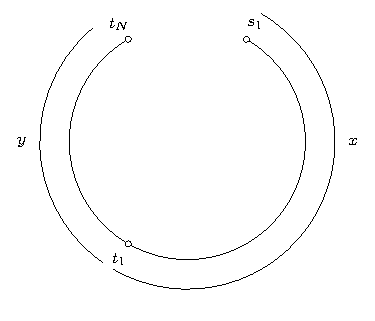
\includegraphics{pictures/lessthan3.pdf}
			\end{subfigure}
			\hspace{50pt}
			\begin{subfigure}[b]{0.3\textwidth}
				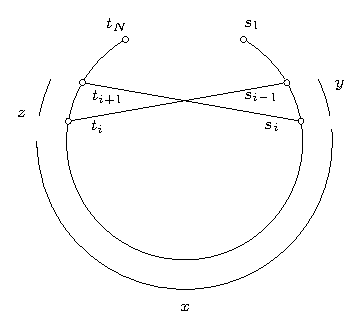
\includegraphics{pictures/lessthan3_2.pdf}
			\end{subfigure}
		\end{center}
		\caption{Illustration for proving the equilibrium must be worse than 3/2.}
		\label{fig:3/2equi}
	\end{figure}    
	
	Since player 1 and $N$ both would not pay more than 3 for the possible solution. Then the rest $N-2$ players must pay at lease $2N-7$. There must exist at lease one player $i$ pays at lease $(2N-7)/(N-2)$. Suppose player $i$ pays $x$ to $s_i \rightarrow t_i$, $y$ to $s_{i-1} \rightarrow s_i$, $z$ to $t_i \rightarrow t_{i+1}$. Possible incentive choices for player $i$ include the choice to pay for only the path from $s_i \rightarrow t_i$, or the path from $s_{i-1} \rightarrow s_i$ and an additional edge $t_{i+1}s_i$,or the path from $t_i \rightarrow t_{i+1}$ and an additional edge $t_is_{i-1}$. Player $i$ has \[max\{\frac{x+y+z}{x},\frac{x+y+z}{1+y},\frac{x+y+z}{1+z}\}\] incentive to deviate. 
	$max\{\frac{x+y+z}{x},\frac{x+y+z}{1+y},\frac{x+y+z}{1+z}\}$ is minimized when $x = 1+y =1+z$. 
		\[x+y+z \geq \frac{2N-7}{N-2}\]
		\[x \geq \frac{4N-11}{3N-6}\]
		\[\frac{x+y+z}{x} \geq \frac{3x-2}{x} = 3-\frac{2}{x} \geq \frac{6N-21}{4N-11} \]
	
		\begin{lemma}
			Given there at least exists a player $i$ needs to pay at least $\frac{2N-7}{N-2}$, we find that player $i$ will at least have the incentive $\frac{6N-21}{4N-11} > \frac{3}{2}$ to deviate.
		\end{lemma}
	
	\subsection{Bicriteria Approximation}
	The following table gives a general result from the paper. Bicriteria approximations, written as $(\beta,\alpha)$, meaning there exists (or it is possible to find) a $\beta$-approximate Nash equilibrium that is only a factor of $\alpha$ more expensive than the centralized optimum.
	\begin{center}
			\begin{tabular} { 
				| m{5cm} | m{3cm}| m{3cm} | }
			   \hline
				& Single Source & Multi-Source\\
			   \hline
			   Exists Nash  & (1,1)  &  (3,1)\\
			  \hline
			  Can find Nash in poly-time & $(1+\epsilon,1.55)$ & $(4.65+\epsilon,2)$\\
			  \hline
			  Lower Bounds on Existence & (1,1) & (1.5,1)\\
			  \hline
			  \end{tabular}
	\end{center}

	The closest approximation ratio had been obtained was 1.55 by k-restricted Steiner Tree. A better approximation ratio, 1.39, was archived 2 years after this paper by modeling Steiner tree into linear programming relaxation and iterative randomized rounding.
	

\begin{thebibliography}{10}
	\setlength{\itemsep}{0pt plus .3pt}
	\setlength{\parsep}{0pt plus .3pt}
	\setlength{\parskip}{0pt plus .3pt}
\bibitem{texbook}
Vazirani Vijay V. {\em Approximation Algorithms.\/} Chapters 3.1 and 22, Springer, 2003.
\end{thebibliography}

\end{document}



